\documentclass[a4paper, 11pt]{article}
\usepackage[utf8]{inputenc}
\usepackage[russian]{babel}
\usepackage{amssymb}
\usepackage{amsmath}
\usepackage{graphicx}
\usepackage{float}

\usepackage{xcolor}

\newcommand{\w}{\widetilde}

\voffset = -1cm 
\footskip=100pt
\hoffset = -1cm

\newcommand{\wide}{
\stackrel{0}{x}
}
\begin{document}
\begin{center}

\textsc{Спектр линеаризированного оператора разностной схемы на стационарном решении
системы уравнений одномерного движения вязкого баротропного газа}

\end{center}

\section{Постановка задачи}
Для разностной схемы с центральными разностями для логарифма плотности построим матрицу
дифференциального оператора на стационарном решении.
Задача - найти собственные значения такого оператора.

\section{Построение оператора}
Для построения, учитывая, что стационарное решение - решение с постоянной плотностью и нулевой скоростью:
\begin{enumerate}
\item Положим $\forall m, n : V_m^n = 0,\ G_m^n = G$, где $G = \ln \rho_0$ и $\rho_0$ - положительная константа.
\item Заменим в схеме $G_m^n$ на $G + J_m$,  $V_m^n$ на $W_m$.
\item Отбросим слагаемые, не зависящие от $J_m$ и $W_m$.
\item Отбросим слагаемые, зависящие нелинейно от $J_m$ и $W_m$.
\item Заменим $e^{_G} = \frac{1}{\rho_0}$.
\end{enumerate}

\newpage

Тогда разностная схема примет вид:
$$
\begin{cases}
\displaystyle{
W_0 \left(-\frac{3}{h}\right) + W_1 \left(\frac{4}{h}\right) + W_2 \left(-\frac{1}{h}\right) = 0,
} & (1)
\\
\\
\displaystyle{
W_{m - 1} \left(-\frac{1}{h}\right) + W_{m + 1} \left(\frac{1}{h}\right) = 0,\ \ \ 1 \leqslant m \leqslant M - 1,
}  & (2)
\\
\\
\displaystyle{
W_{M - 2} \left(\frac{1}{h}\right) + W_{M - 1} \left(-\frac{4}{h}\right) + W_M \left(\frac{3}{h}\right) = 0, 
} & (3)
\\
\\
\displaystyle{
J_{m-1} \left(\frac{\tilde{p}' (\rho_0)}{2h}\right) + J_{m + 1} \left(-\frac{\tilde{p}' (\rho_0)}{2h}\right) + 
W_{m-1} \left(-\frac{\mu}{\rho_0 h^2}\right) + 
} 
\\
\\
\displaystyle{
+ W_m \left(\frac{2\mu}{\rho_0 h^2}\right) +
W_{m+1} \left(-\frac{\mu}{\rho_0 h^2}\right) = 0,\ \ \ 1\leqslant m \leqslant M - 1.
} & (4)
\\
\\
W_0 = 0
\\
\\
W_M = 0
\end{cases}
$$

Отбросим тривиальные $W_0$ и $W_M$ и построим матрицу следующим образом:
\begin{enumerate}
\item Колонкам переменные отвечают в следующем порядке: 

\center {$J_0, J_1, W_1, J_2, \ldots, W_{M-1}, J_M$}

\item Строчки заполняются уравнениями так:
\begin{center}
$$
\begin{pmatrix}
(1) \\ 
(2)\vert_{m = 1} \\
(4)\vert_{m=1} \\
(2)\vert_{m=2} \\
(4)\vert_{m=2} \\
 \vdots \\
(2)\vert_{m=M-1} \\
(4)\vert_{m=M-1} \\ 
(3)
\end{pmatrix}$$
\end{center}
\end{enumerate}

Покажем на комплексной плоскости собственные значения такого оператора для
$$
\begin{cases}
\rho_0 = 1 \\
\tilde{p}' (x) = 1 \\
M = 120 \\
X = 10 \\
h = \frac{1}{12} \\
\mu = 0.01 \\
\end{cases}
$$

\begin{figure}[H]
		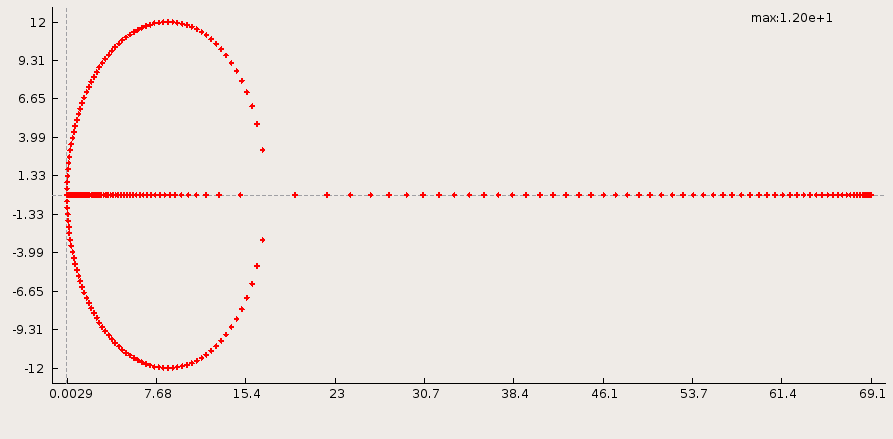
\includegraphics[width=1\linewidth]{plot.png}
\end{figure}
\end{document}
